\chapter{Test of Signal to Noise Ratio on the guitar}\label{app:test:snr}

The test of SNR of the \gls{dsp} is going to be presented in this appendix. It will include the used material and setup, the test procedure and the results. \\

\section{Material and Setup}

In order to perform this test, the following material has been used:

\begin{itemize}
	\item TMS320C5515 eZdsp development board
	\item Analog Discovery Digilent 2 USB Oscilloscope
	\item A computer with Waveforms 2015 and MATLAB
	\item Wires
\end{itemize}


\begin{figure}[htbp!]
\centering
\begin{picture}(0,0)%
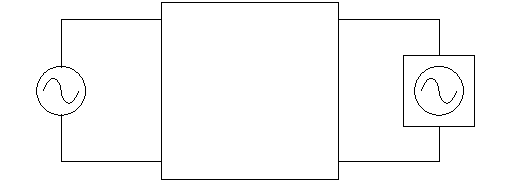
\includegraphics{snr_dsp_test.pdf}%
\end{picture}%
\setlength{\unitlength}{4144sp}%
%
\begingroup\makeatletter\ifx\SetFigFont\undefined%
\gdef\SetFigFont#1#2#3#4#5{%
  \reset@font\fontsize{#1}{#2pt}%
  \fontfamily{#3}\fontseries{#4}\fontshape{#5}%
  \selectfont}%
\fi\endgroup%
\begin{picture}(4044,1374)(-1229,152)
\put(-1214,749){\makebox(0,0)[lb]{\smash{{\SetFigFont{12}{14.4}{\rmdefault}{\mddefault}{\updefault}{\color[rgb]{0,0,0}$V_s$}%
}}}}
\put(2431,749){\makebox(0,0)[lb]{\smash{{\SetFigFont{12}{14.4}{\rmdefault}{\mddefault}{\updefault}{\color[rgb]{0,0,0}Ch2}%
}}}}
\put(541,749){\makebox(0,0)[lb]{\smash{{\SetFigFont{12}{14.4}{\rmdefault}{\mddefault}{\updefault}{\color[rgb]{0,0,0}DSP}%
}}}}
\end{picture}%
\caption{Setup for measuring the \gls{snr} of the \gls{dsp}.}
		\label{fig:appendix:snr_dsp}
\end{figure}


\section{Test Procedure}

\begin{itemize}
	\item Set up the materials as shown in \autoref{fig:appendix:snr_dsp}.
	\item Set the oscilloscope to generate a sine wave of 0.5 V$_{RMS}$ with frequency \SI{1}{\kilo\hertz}.
	\item Measure the output of the \gls{dsp}.
	\item Ground the input of the \gls{dsp}.
	\item Measure the output of the \gls{dsp}.
	\item Calculate the RMS values of the two outputs.
	\item Calculate \gls{snr} using \autoref{eq:snr_dsp}
\end{itemize}

\begin{equation}\label{eq:snr_dsp}
        SNR_{DSP} = 20 \cdot \log_{10}\left(\frac{V_{1RMS}}{V_{2RMS}}\right)
    \end{equation}
    
    \startexplain
    \explain{$SNR_{DSP}$ is the \gls{snr} in the \gls{dsp}.}{\SI{}{\decibel}}
     \explain{$V_{1RMS}$ is the RMS value of the measured output with a sine wave of 0.5 V$_{RMS}$ with frequency \SI{1}{\kilo\hertz} as the input.}{V$_{RMS}$}
     \explain{$V_{2RMS}$ is the RMS value of the measured output with the input grounded.}{V$_{RMS}$}
    \stopexplain
    
V$_{2RMS}$ is calculated by measuring the peak-to-peak of the noise and dividing it by eight. When dividing by eight the noise peak-to-peak value will only exceed this in 0.0006\% of the time \citep{rms_noise}.
V$_{1RMS}$ is calculated by measuring the peak value of the signal and dividing it by $\sqrt{2}$. 

\section{Results}
In \autoref{fig:SNR_dsp_1kHz} the output of the \gls{dsp} with a sine wave of 0.5 V$_{RMS}$ with frequency \SI{1}{\kilo\hertz} as the input is shown. 

\begin{figure}[!h]
  \centering
  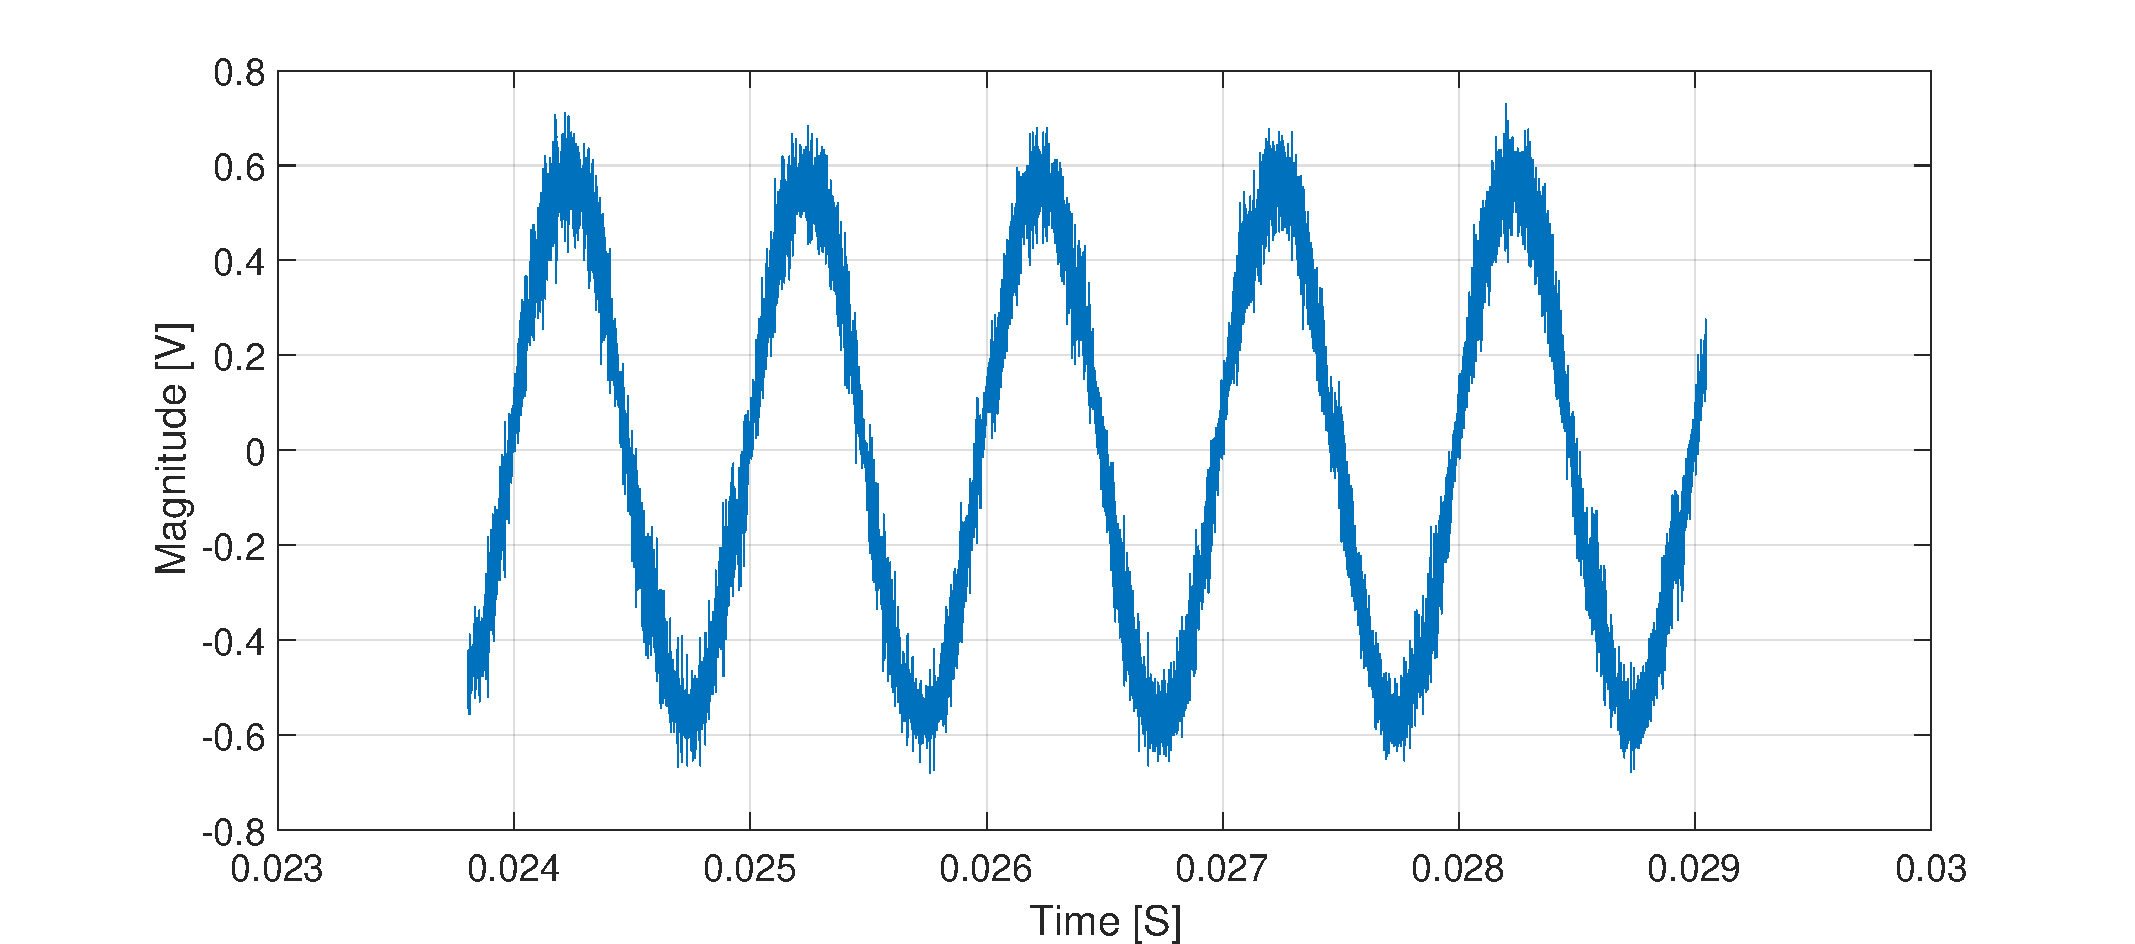
\includegraphics[width=1\textwidth]{SNR_dsp_1kHz.pdf}
  \caption{measured output of the \gls{dsp} with a sine wave of 0.5 V$_{RMS}$ with frequency \SI{1}{\kilo\hertz} as the input.}
  \label{fig:SNR_dsp_1kHz}
\end{figure}

In \autoref{fig:SNR_dsp_gnd} the output of the \gls{dsp} with the input grounded is shown.

\begin{figure}[!h]
  \centering
  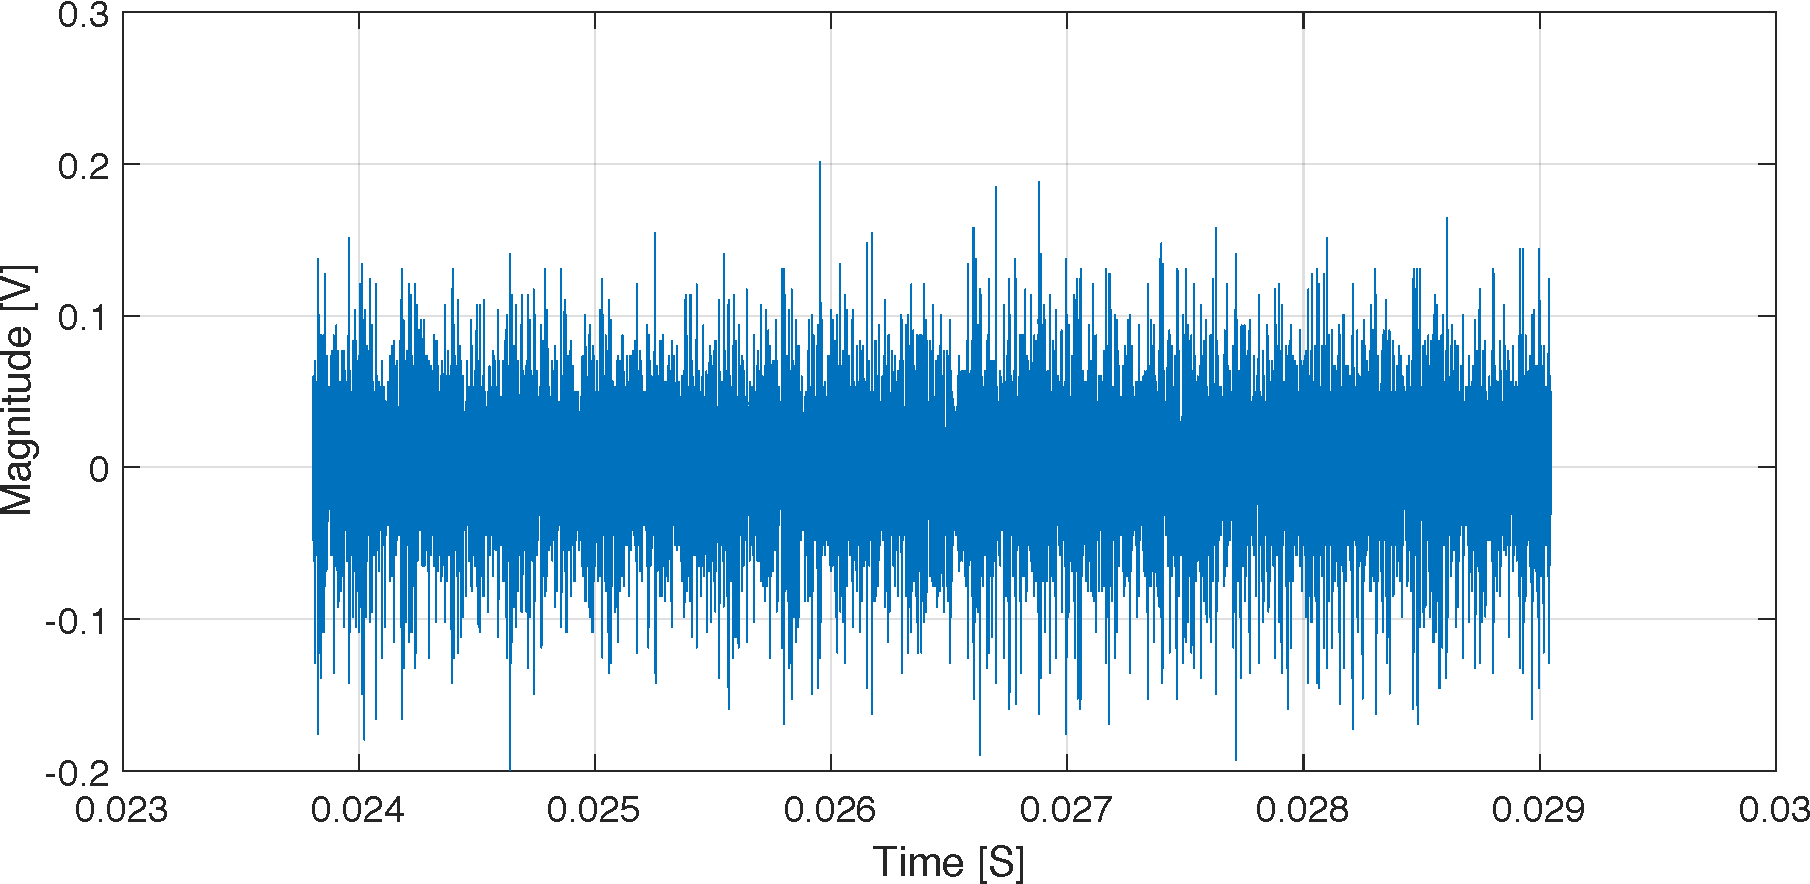
\includegraphics[width=1\textwidth]{SNR_dsp_gnd.pdf}
  \caption{measured output of the \gls{dsp} with the input grounded.}
  \label{fig:SNR_dsp_gnd}
\end{figure}

The peak-to-peak value of \autoref{fig:SNR_dsp_gnd} is \SI{0.4}{\volt}, and thereby $V_{2RMS} = \frac{0.4}{8} = 0.05$ V$_{RMS}$.
The peak value of \autoref{fig:SNR_dsp_1kHz} is measured to be \SI{0.7}{\volt}, and thereby and thereby $V_{1RMS} = \frac{0.7}{\sqrt{2}} = 0.495$ V$_{RMS}$. The \gls{snr} of the \gls{dsp} can thereby be calculated as in \autoref{}.

\begin{equation}\label{eq:snr_dsp_result}
	SNR_{DSP} = 20 \cdot log_{10}\left(\frac{0.495}{0.005}\right) = 39.91dB
	\end{equation}

